\chapter{Probability}\label{Probability}

\section{Introduction}\label{Introduction}

\subsection{Dependent and Independent Variables}\label{Dependent and Independent Variables}
The independent variable is the factor that a researcher manipulates, while the dependent variable is the outcome that is measured to see the effect of the independent variable.

In an experiment, the independent variable is the variable that is changed or controlled to test the effects on the dependent variable. The dependent variable is the variable being tested and measured. For example, in a study to determine the effect of different amounts of sunlight on plant growth, the amount of sunlight is the independent variable, and the growth of the plant is the dependent variable.

Mathematically, if $X$ is the independent variable and $Y$ is the dependent variable, the relationship can be expressed as:
\spacedequation{Y = f(X),}
where $f$ is a function that describes how $Y$ depends on $X$.

In statistical analysis, the relationship between the independent and dependent variables can be analyzed using various methods such as correlation and regression analysis. The correlation coefficient $r$ measures the strength and direction of the linear relationship between two variables:
\spacedequation{r = \frac{\sum (X_i - \bar{X})(Y_i - \bar{Y})}{\sqrt{\sum (X_i - \bar{X})^2 \sum (Y_i - \bar{Y})^2}},}
where $X_i$ and $Y_i$ are the individual sample points, and $\bar{X}$ and $\bar{Y}$ are the means of $X$ and $Y$ respectively.

Regression analysis can be used to model the relationship between the independent and dependent variables. In simple linear regression, the relationship is modeled as:
\spacedequation{Y = \beta_0 + \beta_1 X + \epsilon,}
where $\beta_0$ is the intercept, $\beta_1$ is the slope, and $\epsilon$ is the error term.

More on exact methods to determine the meaning of such relations is discussed later in \textit{statistics}.

\subsection{Kolmogorov's Axioms}\label{Kolmogorov's Axioms}
Kolmogorov's three axioms are the most well-known description of the fundamental properties of probability theory. Let $\Omega = \{\omega_1, \omega_2, \omega_3, \omega_4, \omega_5, \omega_6\}$ be the sample space of a random experiment, $A$ and $B$ subsets of $\Omega$, and $P$ a function that assigns a real number between 0 and 1 to each $A$. $P(A)$ is called probability if the following three conditions (axioms) are met:
\begin{enumerate}
    \item $P(A) \geq 0$: This condition states that the probability of any subset of $\Omega$ (event) is non-negative. This property is also called non-negativity.
    \item $P(\Omega) = 1$: The second axiom further restricts the range of values of the function $P$. With axioms 1 and 2, $P(A)$ can take any value between 0 and 1.
    \item $P(A \cup B) = P(A) + P(B)$ for disjoint sets $A$ and $B$: This means that no outcome satisfies both events. $A$ and $B$ are called disjoint in this case.
\end{enumerate}

\subsection{Probability Concepts}\label{Probability Concepts}

\subsubsection{Probability Formulas}\label{Probability Formulas}

In probability theory, there are various concepts that help us understand the relationships between different events or variables. These include joint probability, marginal probability, and conditional probability. The joint probability $P(X, Y)$ gives the probability that both event X and event Y occur. It can be calculated by multiplying the conditional probability of one event given the other by the probability of the other event:

\spacedequation{P(X, Y) = P(X|Y) \cdot P(Y) = P(Y|X) \cdot P(X).}

The marginal probability (in English \textbf{marginal} or \textbf{total probability}) $P(X)$ is the probability that event X occurs, regardless of other events. It can be calculated by summing the joint probabilities over all possible values of Y:

\spacedequation{P(X) = \sum_{y} P(X, Y=y) = \sum_{y} P(X|Y=y) \cdot P(Y=y).}

The conditional probability $P(X|Y)$ gives the probability that event X occurs given that event Y has occurred. It can be calculated by dividing the joint probability of X and Y by the probability of Y:

\spacedequation{P(X|Y) = \frac{P(X, Y)}{P(Y)}.}

If a third variable Z is present, these formulas can be extended to calculate conditional and joint probabilities considering Z. For example, the joint probability of X and Y given Z is defined as:

\spacedequation{P(X, Y|Z) = P(X|Y, Z) \cdot P(Y|Z) = P(Y|X, Z) \cdot P(X|Z).}

And the conditional probability of X given Y and Z is defined as:

\spacedequation{P(X|Y, Z) = \frac{P(X, Y|Z)}{P(Y|Z)}}

with $Y$ and $Z$ being variable.

\subsubsection{Conditional Independence}\label{Conditional Independence} 
Conditional independence occurs when the occurrence of event X has no effect on the probability of event Y given event Z. In other words, X and Y are conditionally independent if the conditional probability of Y given X and Z is equal to the conditional probability of Y given Z. This is mathematically expressed by the equation 
\spacedequation{P(Y|X,Z) = P(Y|Z).}
If X and Y are independent given Z, it is written as 
\spacedequation{P(X,Y|Z) = P(X|Z) \cdot P(Y|Z).}

\subsubsection{Independence of Variables}\label{Independence of Variables} 
Two variables X and Y are independent if the occurrence of one variable has no effect on the probability of the occurrence of the other variable. Mathematically, this means that the joint probability of X and Y is equal to the product of the individual probabilities of X and Y:
\spacedequation{P(X,Y) = P(X) \cdot P(Y).}
If X and Y are independent, it also holds that \spacedequation{P(X|Y) = P(X)} and \spacedequation{P(Y|X) = P(Y).}

\section{Probability Distributions}\label{Probability Distributions}
Probability distributions describe how probabilities are assigned to different outcomes of a random variable. They are categorized into discrete and continuous types.

A \textbf{Discrete Random Variable} has a finite or countable number of possible values, such as the outcomes of a coin toss or a die roll.

A \textbf{Continuous Random Variable} has an infinite number of possible values within a given range, such as hair length measured with increasing precision.

The \textbf{Probability Density Function} (PDF) describes the likelihood of a continuous random variable taking on a particular value. The total area under the PDF curve is 1, representing the total probability. Since the probability of a single value is effectively zero, probabilities are calculated over intervals using integration, resulting in the cumulative distribution function (CDF).

Key concepts include the expected value $E$, variance $V$ (with standard deviation $\sqrt{V}$), and the PDF.

\section{Continuous Probability Distributions}\label{Continuous Probability Distributions}

\subsection{Normal Distribution}\label{Normal Distribution}
The normal distribution is also called the Gaussian bell curve. The two parameters ($\mu$ and $\sigma$) represent the mean and standard deviation of the normal distribution. The central limit theorem states that under certain general conditions, the sum of n independent, identically distributed random variables is again normally distributed.

As an example, let's consider rolling n fair dice: If you roll only one die, each face value is equally likely. However, if you roll n dice, the average face value is described by the normal distribution.

Therefore, the normal distribution is the most important, as natural phenomena with sufficiently large n approximate it. The formula for calculating the distribution is:
\spacedequation{f(x,\mu, \sigma) = \frac{1}{\sigma \sqrt{2\pi}} \cdot e^{-\frac{1}{2} \left( \frac{x - \mu}{\sigma} \right)^2}.}

It holds that $E=\mu$ and $V=\sigma^2$ (variance $V$ and standard deviation $\sigma$). The total area enclosed by the curve of the normal distribution is always 1. If $\mu=0$ and $\sigma=1$, it is called the standard normal distribution, which is described by a simplified equation (since $\mu=0$ and $\sigma=1$):
\spacedequation{f(x) = \frac{1}{\sqrt{2\pi}} e^{-\frac{1}{2} x^2}.}

The prefactor ensures that the total area under the curve (and thus the integral from $-\infty$ to $\infty$) is exactly 1. The $\frac{1}{2}$ in the exponent of the exponential function gives the normal distribution a unit variance. Every normal distribution is a variant of the standard normal distribution with scaled standard deviation ($\frac{1}{\sigma}$) and \textit{z-transformed} $\frac{x - \mu}{\sigma}$. The normal distribution is usually written as: $\mathcal{N}(\mu, \sigma^2)$.

\begin{figure}[h]
    \centering
    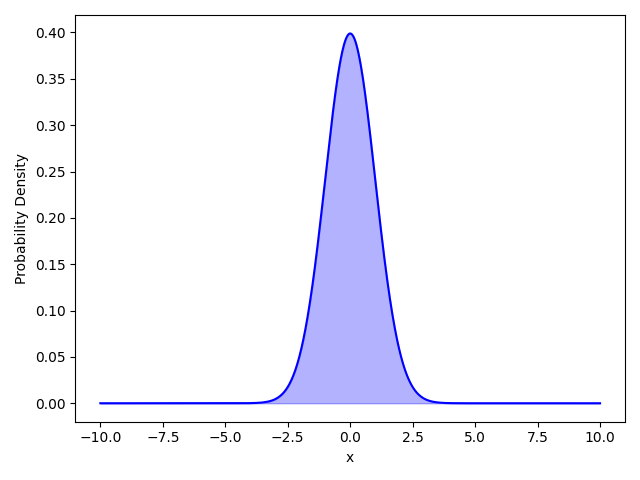
\includegraphics[width=0.5\textwidth]{../images/plot_normal_distribution.png}
    \caption{Normal Distribution with $\mu=0$ and $\sigma=1$}
    \label{fig:normal_distribution}
\end{figure}


\subsubsection{Mixed Distribution}\label{Mixed Distribution}
A mixed distribution consists of several subsets that together form a larger distribution. Such an approach can be used to model a large population with different subpopulations, each of which has individual characteristics. Formally, for each subpopulation $z$, a specific distribution $P(X\mid Z=z)$ is provided. These are mixed according to the probability $P(Z=z)$ of selecting an individual from this subpopulation, i.e.,
\spacedequation{P(X=x) = \sum_{z} P(Z=z)\cdot P(X=x\mid Z=z).}

\begin{figure}[h]
    \centering
    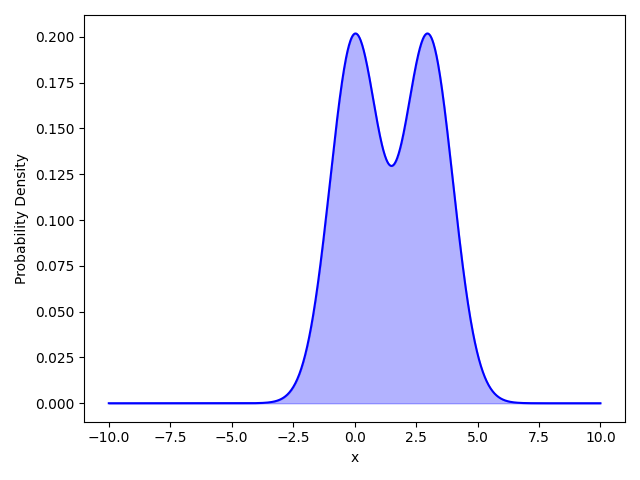
\includegraphics[width=0.5\textwidth]{../images/plot_mixed_normal_distribution.png}
    \caption{Mixed Normal Distribution}
    \label{fig:mixed_normal_distribution}
\end{figure}

\subsubsection{t-Distribution or Student's t-Distribution}\label{t-Distribution or Student's t-Distribution}
The t-distribution, also known as Student's t-distribution, is used in statistical procedures when the sample size is small and the population standard deviation is unknown. It compensates for the underestimation of the standard deviation by the normal distribution in such cases. The t-distribution has wider tails than the normal distribution, which accounts for the increased variability in smaller samples. As the sample size increases, the t-distribution approaches the normal distribution.

The t-distribution is defined as:
\spacedequation{T = \frac{Z}{\sqrt{V/\nu}},}
where $Z$ is a standard normal variable, $V$ is a chi-squared variable with $\nu$ degrees of freedom, and $T$ has an expected value $E=0$ and variance $V=\frac{\nu}{\nu-2}$.

\subsubsection{Cauchy Distribution}\label{Cauchy Distribution}
The Cauchy distribution, also known as the Lorentz distribution, is a continuous probability distribution with heavy tails and undefined mean and variance, often used in physics and spectroscopy. Unlike the normal distribution, the Cauchy distribution does not have a finite mean or variance, which makes it distinct in its applications and properties.

\begin{figure}[h]
    \centering
    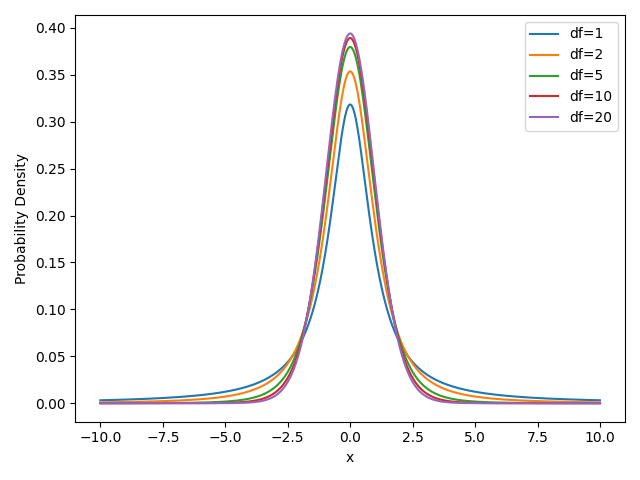
\includegraphics[width=0.5\textwidth]{../images/plot_t_distributions_overlayed.png}
    \caption{t-Distribution}
    \label{fig:t_distribution}
\end{figure}

\subsection{Exponential Distribution}\label{Exponential Distribution}
The exponential distribution is a continuous distribution used to model the duration of random time intervals. The parameter $\lambda$ represents the number of expected \textit{events} per time interval. Examples include the length of a telephone call or radioactive decay. The distribution does not allow negative values, as negative times are meaningless. It is often abbreviated as $\exp(\lambda)$ in statistics. The density function is defined as follows:
\spacedequation{
f_{\lambda}(x) =
\begin{cases}
    \lambda e^{-\lambda x} & \text{if } x \geq 0 \\
    0 & \text{if } x < 0 \\
\end{cases}
}
The expected value $E$ is defined as $\frac{1}{\lambda}$, the variance $V$ as $\frac{1}{\lambda^2}$. The mode (the value at which the probability is highest) of this density function is at $x_{\text{mod}}=0$. If you wish to calculate the probability of the occurrence of an event, it is ideal to use the cumulative distribution function $F(x)$, which forms the integral up to a value $x$. This creates an accumulated probability $P(X\leq x)$. Often, the actual distribution is not an exponential distribution, but the exponential distribution is easy to handle and is applied for simplification. It is applicable when a Poisson process is present, i.e., the Poisson assumptions are fulfilled. The exponential distribution is part of the much larger and more general exponential family, a class of probability measures characterized by ease of handling.

\begin{figure}[h]
    \centering
    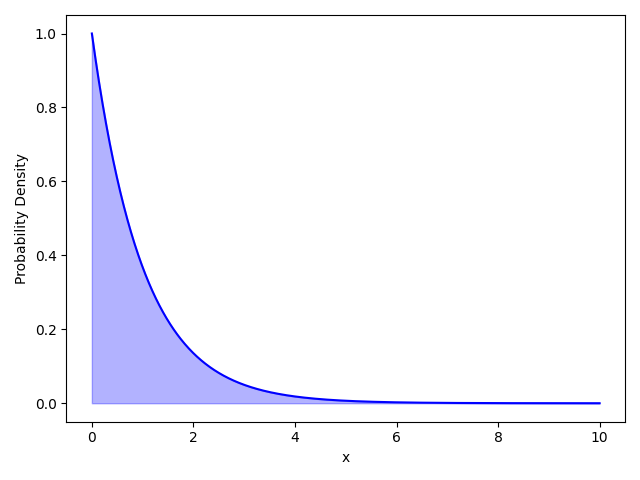
\includegraphics[width=0.5\textwidth]{../images/plot_exponential_distribution.png}
    \caption{Exponential Distribution}
    \label{fig:exponential_distribution}
\end{figure}

\subsubsection{Poisson Distribution}\label{Poisson Distribution}
The Poisson distribution is a discrete probability distribution that describes the distribution of count data. In other words, how often does a certain countable event occur if it is repeated very often? The parameter here indicates the average event rate. The probability for the random variable $X$ of the Poisson distribution is calculated using the following formula:
\spacedequation{P(X=x) = \frac{\lambda^x}{x!} \cdot e^{-\lambda}, \quad x \in \mathbb{N}_0.}
There is a connection between the exponential distribution and the Poisson distribution. Both consider the same phenomenon from different perspectives. The exponential distribution indicates how the probability of the duration of various processes is distributed. The Poisson distribution counts how often the counted events occur in a fixed interval. Starting from the exponential distribution, one wants to determine the probability that exactly $n$ events occur in a time interval of $t$. As will be shown, the result is the Poisson distribution. Since the binomial coefficient for larger values can only be calculated with increased computational effort, one can use the Poisson distribution to approximate the binomial distribution. The Poisson distribution is generally used to approximate the binomial distribution when $n$ is large and $p$ is small. For the expected value $E=\mu$ of the Poisson distribution, we use $\mu=\lambda=n \cdot p$, which is identical to the variance. In general, the Poisson distribution approximates the binomial distribution very well for values of $n \geq 100$ and $\lambda \leq 10$. In addition to the speed advantages in calculation, the Poisson distribution has the advantage that it is countably infinite, thus extending into positive infinity.

\begin{figure}[h]
    \centering
    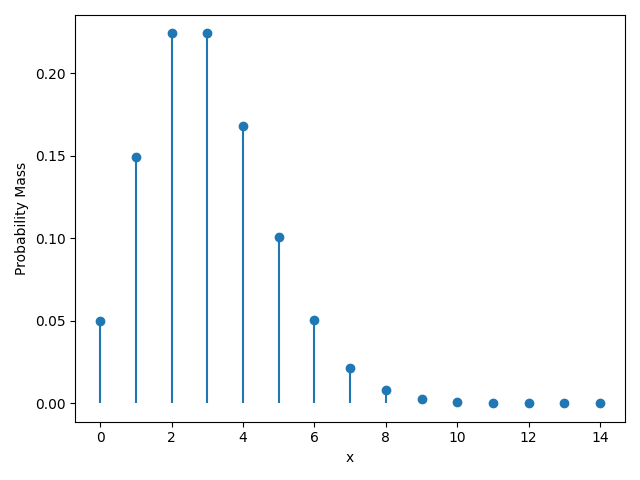
\includegraphics[width=0.5\textwidth]{../images/plot_poisson_distribution.png}
    \caption{Poisson Distribution}
    \label{fig:poisson_distribution}
\end{figure}

\subsubsection{Gamma Distribution}\label{Gamma Distribution}
The gamma distribution is a continuous probability distribution that generalizes the exponential distribution by introducing a shape parameter $\alpha$ and a rate parameter $\beta$. It is often used to model waiting times for multiple events in a Poisson process. The gamma distribution is defined by the following probability density function (PDF):

\spacedequation{
f(x; \alpha, \beta) = \frac{\beta^\alpha x^{\alpha-1} e^{-\beta x}}{\Gamma(\alpha)}, \quad x > 0,
}
where $\Gamma(\alpha)$ is the gamma function, which generalizes the factorial function to non-integer values. The expected value $E$ and variance $V$ of the gamma distribution are given by:

\spacedequation{E = \frac{\alpha}{\beta}, \quad V = \frac{\alpha}{\beta^2}.}

The gamma distribution is particularly useful in Bayesian statistics and reliability engineering, where it is used to model the time until failure of systems with multiple components.

\begin{figure}[h]
    \centering
    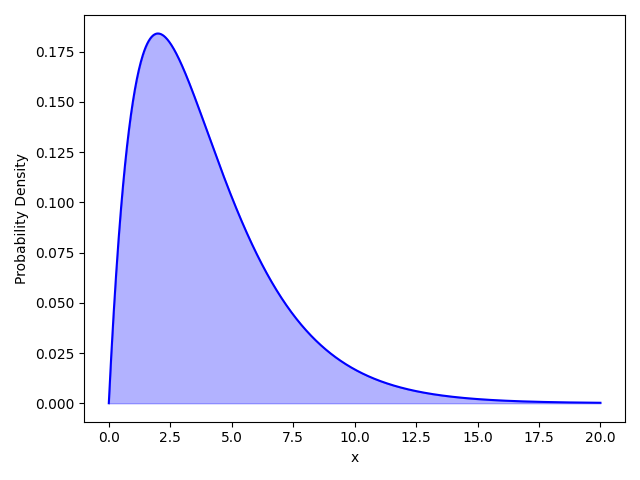
\includegraphics[width=0.5\textwidth]{../images/plot_gamma_distribution.png}
    \caption{Gamma Distribution with $\alpha=2$ and $\beta=1$}
    \label{fig:gamma_distribution}
\end{figure}

\subsubsection{Beta Distribution}\label{Beta Distribution}
The beta distribution is a continuous probability distribution defined on the interval [0, 1], making it suitable for modeling proportions and probabilities. It is characterized by two shape parameters, $\alpha$ and $\beta$, which determine the distribution's shape. The probability density function (PDF) of the beta distribution is given by:

\spacedequation{
f(x; \alpha, \beta) = \frac{x^{\alpha-1} (1-x)^{\beta-1}}{B(\alpha, \beta)}, \quad 0 \leq x \leq 1,
}
where $B(\alpha, \beta)$ is the beta function, which serves as a normalization constant. The expected value $E$ and variance $V$ of the beta distribution are given by:

\spacedequation{E = \frac{\alpha}{\alpha + \beta}, \quad V = \frac{\alpha \beta}{(\alpha + \beta)^2 (\alpha + \beta + 1)}.}

The beta distribution is widely used in Bayesian statistics, particularly as a prior distribution for binomial proportions. It is also used in project management for modeling task completion times and in various fields where probabilities and proportions are analyzed.

\begin{figure}[h]
    \centering
    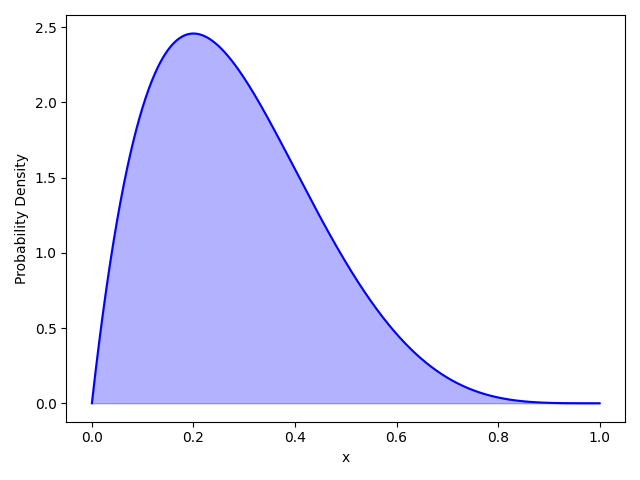
\includegraphics[width=0.5\textwidth]{../images/plot_beta_distribution.png}
    \caption{Beta Distribution with $\alpha=2$ and $\beta=5$}
    \label{fig:beta_distribution}
\end{figure}

\subsubsection{$\chi^2$ Distribution}\label{Chi Square Distribution}
The $\chi^2$ distribution is a continuous distribution often used for testing statistical independence or the validity of a hypothesis (goodness of fit), such as in the \textit{Pearson's chi-square test}~\ref{Pearson's chi-square test}. Very few real-world phenomena are well described by the $\chi^2$ distribution. There is a parameter that defines the degrees of freedom $n$\footnote{If one were to take random independent samples of $n$ normally distributed quantities, these samples would sum to a $\chi^2$ distribution with $n$ degrees of freedom.}. These degrees of freedom determine the distribution insofar as
\spacedequation{\chi_n^2 = Z_1^2 + \dots + Z_n^2}
holds, meaning that $n$ independent, squared, and standard normally distributed random variables are approximately equivalent to it, that is,
\spacedequation{Z_k \sim \mathcal{N}(0,1) \quad \forall k = 1,\dots,n}
and
\spacedequation{\chi^2 \sim \chi_n^2.}
It also holds that
\spacedequation{E_{\chi^2} = n}
and
\spacedequation{V_{\chi^2} = 2 \cdot n.}

\begin{figure}[h]
    \centering
    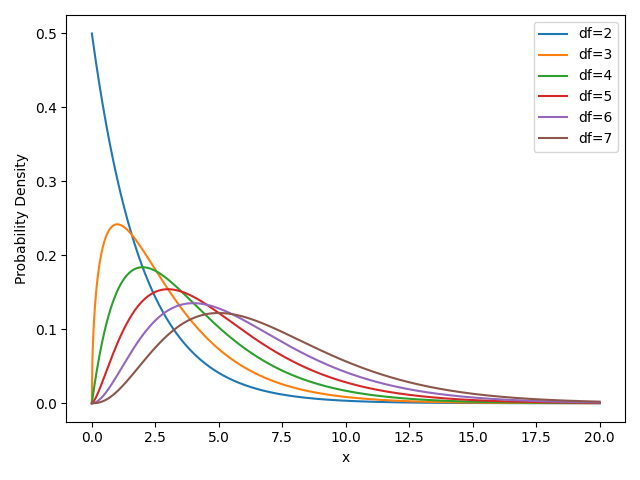
\includegraphics[width=0.5\textwidth]{../images/plot_chi_squared_overlayed.png}
    \caption{$\chi^2$ Distribution}
    \label{fig:chi_square_distribution}
\end{figure}

\subsection{Uniform Distribution}\label{Uniform Distribution}
The French mathematician Pierre Simon de Laplace (1749 to 1827) was one of the first to intensively study random experiments in which it can be assumed that each of its outcomes occurs with the same probability. Random experiments with uniform distribution are called Laplace experiments. The uniform distribution is a special case among probability distributions, as it exists both as a \textit{continuous} and as a \textit{discrete} distribution. Here are briefly the formulas for their calculation. First, for the case of a discrete distribution:
\spacedequation{f(x)=\frac{1}{n}, \quad E(x)=\frac{n+1}{2}, \quad V(x)=\frac{1}{n}\sum_{i=0}^{n}(x_i-\mu)^2.}
And for a continuous distribution:
\spacedequation{
f(x)=
\begin{cases}
    \frac{1}{b-a} & \text{if } a \leq x \leq b \\
    0 & \text{otherwise}. \\
\end{cases}
}
Here, $a$ and $b$ are the boundaries of an interval that includes $x$. Since the same probability applies to all $x$, this depends on the boundaries of the interval
\spacedequation{E(x)=\frac{a+b}{2}, \quad V(x)=\frac{1}{12}(b-a)^2.}

\begin{figure}[h]
    \centering
    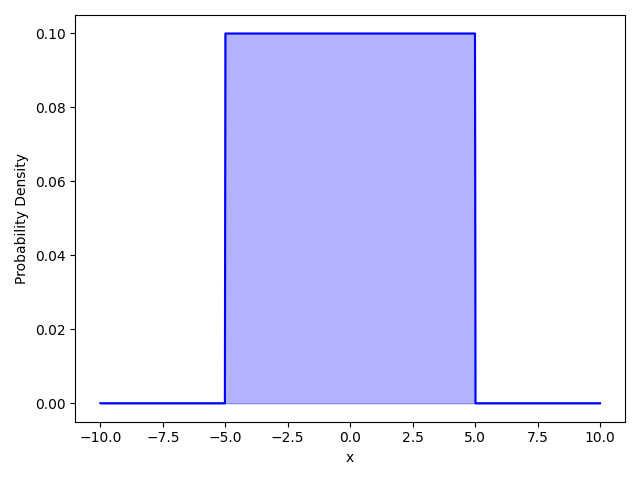
\includegraphics[width=0.5\textwidth]{../images/plot_uniform_distribution.png}
    \caption{Uniform Distribution}
    \label{fig:uniform_distribution}
\end{figure}

\section{Discrete Distributions}\label{Discrete Distributions}
\subsubsection{Binomial Distribution}\label{Binomial Distribution}
Processes in which only two possible outcomes are conceivable (e.g., a coin toss) can be described with the binomial distribution. A prerequisite is that the experiment consists of identical and independent trials. The parameters $n$ and $k$ suggest that this is a discrete probability distribution that answers questions about $k$ successes in $n$ trials. It holds:

\spacedequation{
\begin{tabular}{|c|c|}
    \hline
    Variable & Formula \\
    \hline
    $P(X = k)$ & $\binom{n}{k} p^k (1 - p)^{n - k}$ \\
    $E$ & $n p$ \\
    $V$ & $n p q$ \\
    $\sigma$ & $\sqrt{n p q}$ \\
    $\binom{n}{k}$ & $\dfrac{n!}{k! (n - k)!}$ \\
    \hline
\end{tabular}
}

The binomial coefficient describes the number of ways in which $k$ objects can be arranged in a group of $n$ without repetition. The binomial distribution is left-skewed when $p > 0.5$\footnote{Greater than but not equal to! Symbol missing.}, right-skewed when $p < 0.5$, and symmetric when $p = 0.5$. When $n$ is sufficiently large, the normal distribution can be used as an approximation to the binomial distribution, as the skewness decreases with increasing $n$.

\begin{figure}[h]
    \centering
    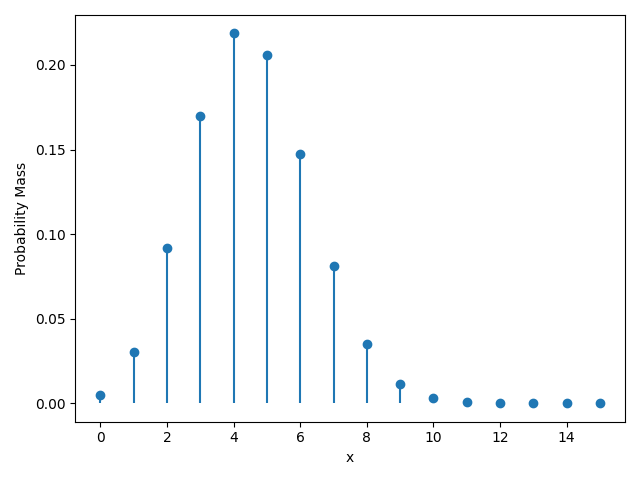
\includegraphics[width=0.5\textwidth]{../images/plot_binomial_distribution.png}
    \caption{Binomial Distribution with $n=15$ and $p=0.3$}
    \label{fig:binomial_distribution}
\end{figure}

\subsubsection{Bernoulli Distribution}\label{Bernoulli}
The Bernoulli distribution is a discrete distribution whose random variable $X$ takes only two values: 0 (failure) or 1 (success). It arises when performing a Bernoulli experiment (which has only two possible outcomes) exactly once. The Bernoulli distribution is therefore a special case of the binomial distribution for $n = 1$.

It holds:
\spacedequation{E_{\text{Bernoulli}} = p,}
\spacedequation{V_{\text{Bernoulli}} = p (1 - p),}
and
\spacedequation{
f_{\text{Bernoulli}}(x) = \begin{cases}
    1 - p & \text{if } x = 0 \\
    p & \text{if } x = 1 \\
    0 & \text{otherwise}. \\
\end{cases}
}

\begin{figure}[h]
    \centering
    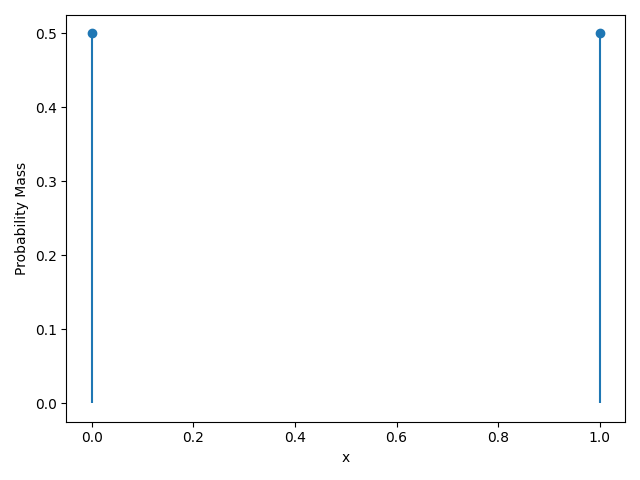
\includegraphics[width=0.5\textwidth]{../images/plot_bernoulli_distribution.png}
    \caption{Bernoulli Distribution with $p=0.5$}
    \label{fig:bernoulli_distribution}
\end{figure}



\section{Maximum Likelihood Estimation}\label{Maximum Likelihood Estimation}
Maximum Likelihood Estimation (MLE) is a method used to estimate the parameters of a statistical model. It works by finding the parameter values that maximize the likelihood function, which measures how well the model explains the observed data. The purpose of MLE is to provide the most likely estimates of the model parameters based on the given data.

The likelihood function $L(\theta)$ for a set of observations $X = \{x_1, x_2, \ldots, x_n\}$ is defined as the joint probability of the observations given the parameters $\theta$:
\spacedequation{L(\theta) = P(X|\theta) = \prod_{i=1}^{n} P(x_i|\theta).}

To find the MLE, we take the natural logarithm of the likelihood function, known as the log-likelihood function $\ell(\theta)$, and then find the parameter values that maximize it:
\spacedequation{\ell(\theta) = \log L(\theta) = \sum_{i=1}^{n} \log P(x_i|\theta).}

The MLE $\hat{\theta}$ is the value of $\theta$ that maximizes $\ell(\theta)$:
\spacedequation{\hat{\theta} = \arg \max_{\theta} \ell(\theta).}

To illustrate MLE, take a look at an animation that shows how the likelihood function changes as the parameter values are adjusted: execute the script found here: \href{../scripts/mle_viz.py}{mle\_viz.py}

\section{Bayes}\label{Bayes}
Bayes' theorem makes statements about probabilities given that one knows data or observations, moving from events ($Data$) to their causes (parameters $\Theta$). The more data there is, the more reliable the probability distribution of a variable becomes. Bayes' theorem states:

\spacedequation{P(\Theta|Data) = \frac{P(Data|\Theta) \cdot P(\Theta)}{P(Data)}.}

Here, $P(\Theta|Data)$ is the \textbf{posterior} probability of the parameters given the data. $P(Data|\Theta)$ is the \textbf{likelihood} of observing the data given the parameters. For $P(\Theta)$, one usually sets a \textbf{prior}, that is, its probabilities without prior knowledge.

Let us consider the so-called "Monty Hall Problem". In this game, there are three doors, behind one of which is a prize, and behind the other two are goats. The player selects a door, and the host opens another door behind which there is a goat. The player then has the option to stay with their original choice or to switch. The question is: Should the player stay with their original choice? Using Bayes' theorem, this question can be clearly answered.

Let $A$ be the chosen door and $C$ the door that the host opens. What is the probability that the prize is behind door $A$, given that $C$ was opened, and what is it for door $B$? \textbf{\textit{We need to calculate $P(A|C)$ and $P(B|C)$.}} If $P(B|C) > P(A|C)$, one should switch! We know that $P(A) = P(B) = P(C) = \dfrac{1}{3}$, and that only one door is opened behind which there is not the prize. It holds:

\spacedequation{P(A|C) = \frac{P(C|A) \cdot P(A)}{P(C)} = \frac{P(C|A) \cdot P(A)}{P(C|A) \cdot P(A) + P(C|B) \cdot P(B) + P(C|C) \cdot P(C)},}

where $P(C)$ normalizes the probabilities according to the principle of total probability (the sum of all probabilities under which $C$ is opened in our case). Substituting the values, we obtain:

\spacedequation{P(A|C) = \frac{0.5 \cdot \dfrac{1}{3}}{0.5 \cdot \dfrac{1}{3} + 1 \cdot \dfrac{1}{3} + 0 \cdot \dfrac{1}{3}} = \dfrac{1}{3}.}

To understand the logic, ask the question: \textit{How likely is it to open door $X$, given that the prize is behind door $Y$?} On the other hand:

\spacedequation{P(B|C) = \frac{P(C|B) \cdot P(B)}{P(C)} = \frac{P(C|B) \cdot P(B)}{P(C|B) \cdot P(B) + P(C|A) \cdot P(A) + P(C|C) \cdot P(C)}}

\spacedequation{= \frac{1 \cdot \dfrac{1}{3}}{1 \cdot \dfrac{1}{3} + 0.5 \cdot \dfrac{1}{3} + 0 \cdot \dfrac{1}{3}} = \dfrac{2}{3}}

And thus greater for $B$, so one should switch.

Therefore, using Bayes' theorem, we find that the probability of winning by switching doors is $\dfrac{2}{3}$, while the probability of winning by staying is only $\dfrac{1}{3}$. This counterintuitive result demonstrates the power of Bayesian reasoning in updating probabilities based on new information.

Bayes' theorem is widely used in various fields such as statistics, machine learning, medicine, and engineering. It allows for the updating of beliefs in light of new evidence, making it a fundamental tool for probabilistic inference.

In practical applications, Bayes' theorem helps in situations where one needs to determine the probability of a hypothesis given observed data. For example, in medical diagnostics, Bayes' theorem can be used to calculate the probability of a disease given a positive test result, taking into account the prior probability of the disease and the accuracy of the test.

Bayesian methods also play a crucial role in modern data science and machine learning algorithms, such as Bayesian networks and Bayesian inference, which provide a probabilistic approach to reasoning under uncertainty.


